\section{Ovládání západky a IR komunikace}

Zapojení je dostupná na obrázku \ref{fig:E4-sch_IR-Motor-enkoder}

\paragraph{IR komunikace}
\addcontentsline{toc}{paragraph}{IR komunikace}
IR slouží primárně pro identifikaci dveří, při vkládání většího množství dveří do stejného trezoru.
Trezor totiž počítá s možností vkládání více dveří do jednoho trezoru, což je jedna ze schopností, kterou více použije trezor jako hračka, než trezor jako bezpečnostní schránka.
Tento trezor s více dveřmi by zároveň mohl sloužit jako jakýsi displej a na to potřebuje vědět, které dveře jsou kde, na což slouží právě IR komunikace. %todo ???? 

Jako IR přijímač jsem z nabídky JLCPCB \parencite{jlcpcb} zvolil \href{https://datasheet.lcsc.com/szlcsc/1912111437_Everlight-Elec-IRM-H936-TR2_C264266.pdf}{IRM-H936} \parencite{irm-h936}. 
V nabídce JLCPCB jsou v této době jen tři IR-přijímače, jeden z nich je THT a~je~namířen rovnoběžně s deskou a z tohoto důvodu nevyhovuje. 
Druhé dva jsou právě IRM-H936 a \href{https://datasheet.lcsc.com/szlcsc/2010221806_Everlight-Elec-IRM-H638T-TR2-DX_C390031.pdf}{IRM-H638},
z nichž IRM-H936 má skoro poloviční výšku a širší úhel záběru, a to byl důvod jeho volby.

Druhou částí IR komunikace je vysílač, který je zajištěn jednoduše IR ledkou.

\begin{figure}[htbp]
    \centering
    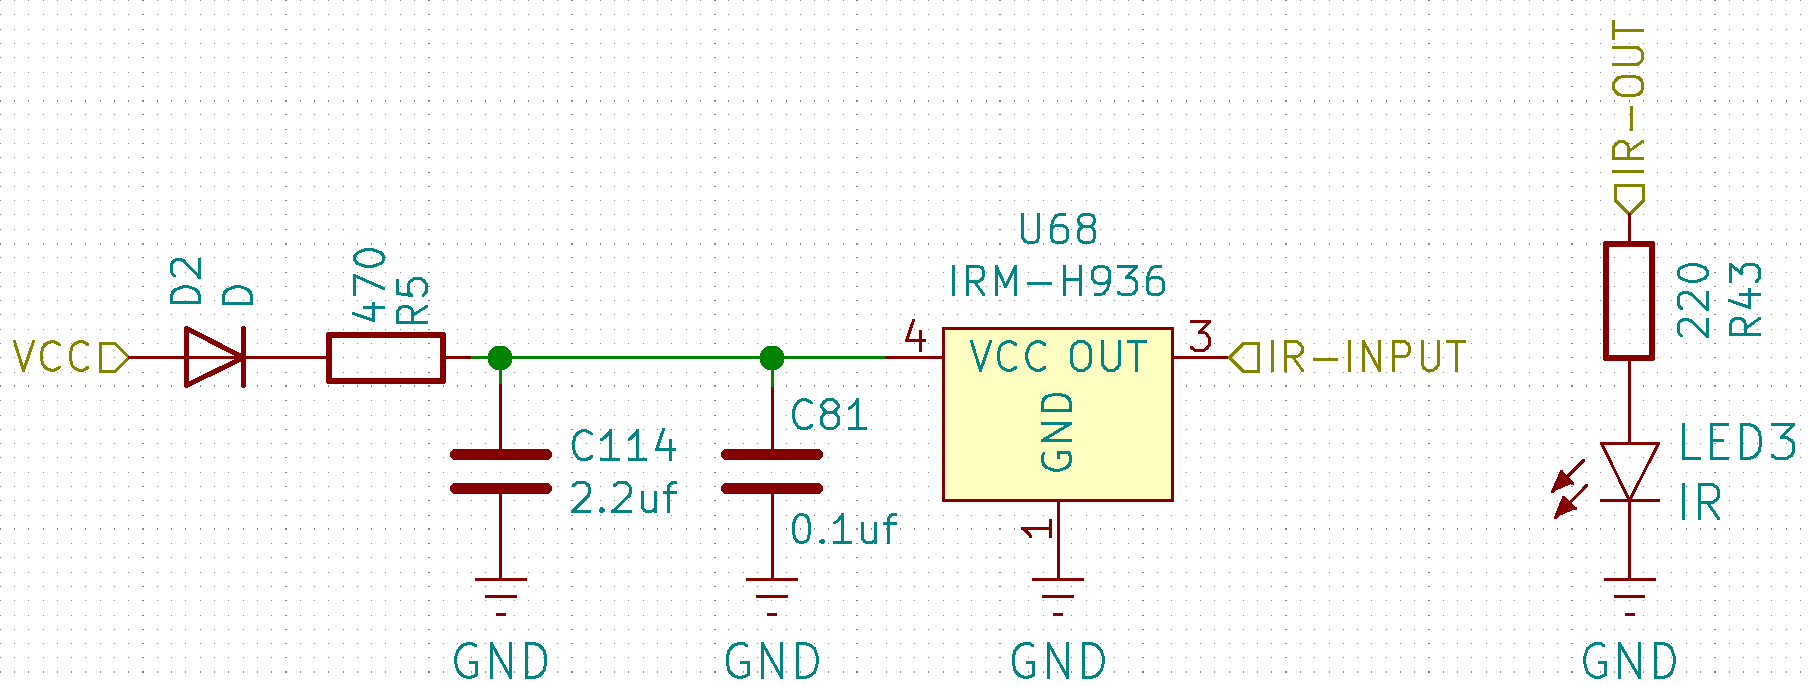
\includegraphics[width=\textwidth]{kapitoly/obrazky/E4/ir_motor_enkoder/IR.png}
    \caption{Zapojení IR vysílače a přijímače}
    \label{fig:E4-ir}
\end{figure}

\newpage

\paragraph{Ovládání motoru}
\addcontentsline{toc}{paragraph}{Ovládání motoru}
Protože motor je napájen z 5~V větve a protože ho připínám k napájení, a ne k zemi, nemůžu ho ovládat přímo z procesoru, proto je Q7 napojen na Q10, který je teprve řízen z~ESP. 
Kvůli napěťovým špičkám, které při běhu vznikají na komutátoru motoru, je zde i zpětná Schottkyho dioda, D3.% D3 skrz sebe propustí záporné napětí, které muže na vzniknout motoru.

\begin{figure}[htbp]
    \centering
    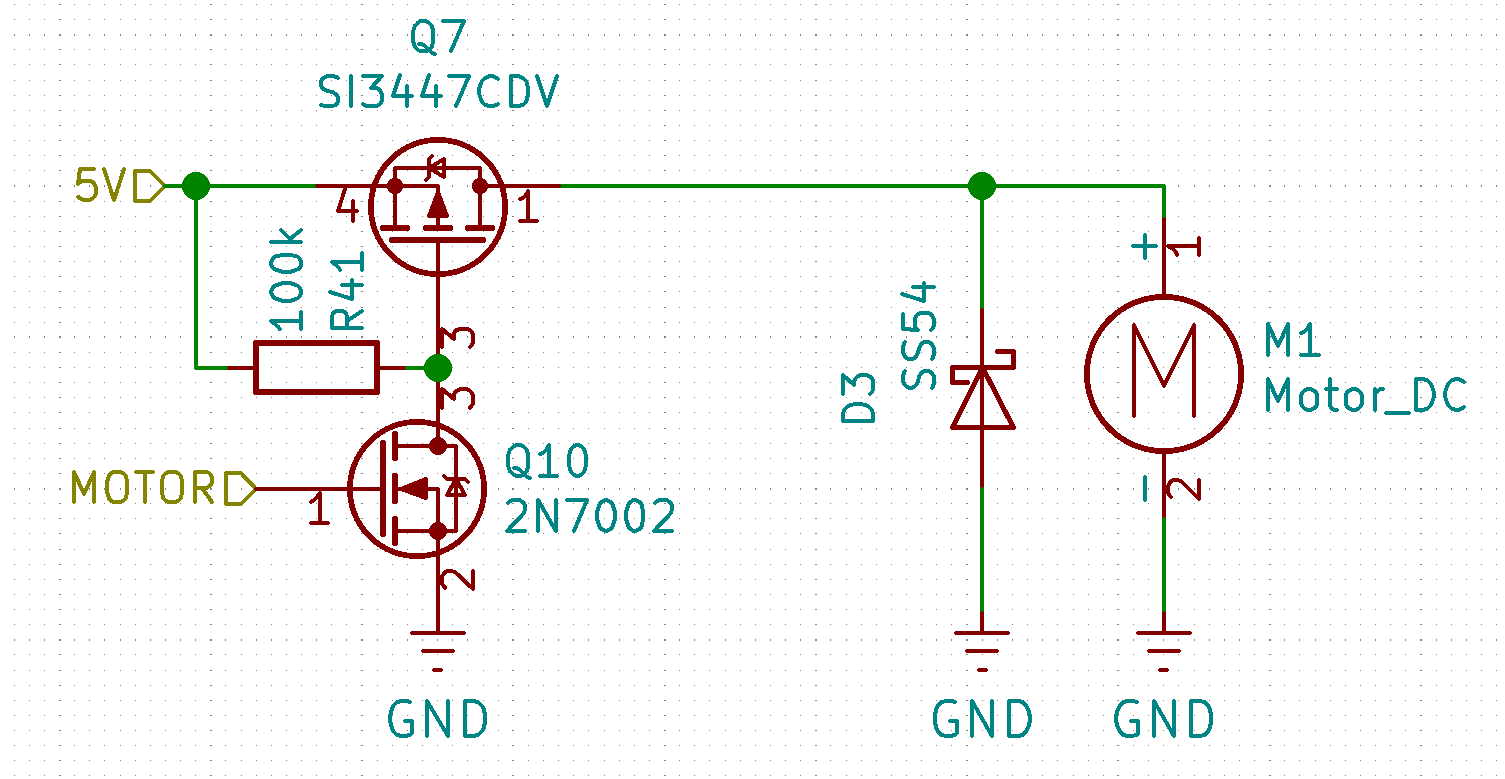
\includegraphics[width=\textwidth]{kapitoly/obrazky/E4/ir_motor_enkoder/ovladani_motoru.png}
    \caption{Zapojení řízení motoru}
    \label{fig:E4-motor}
\end{figure}

\newpage

\paragraph{Enkodér}
\addcontentsline{toc}{paragraph}{Enkoder}

\begin{wrapfigure}[13]{R}{0.65\textwidth}
    \centering
    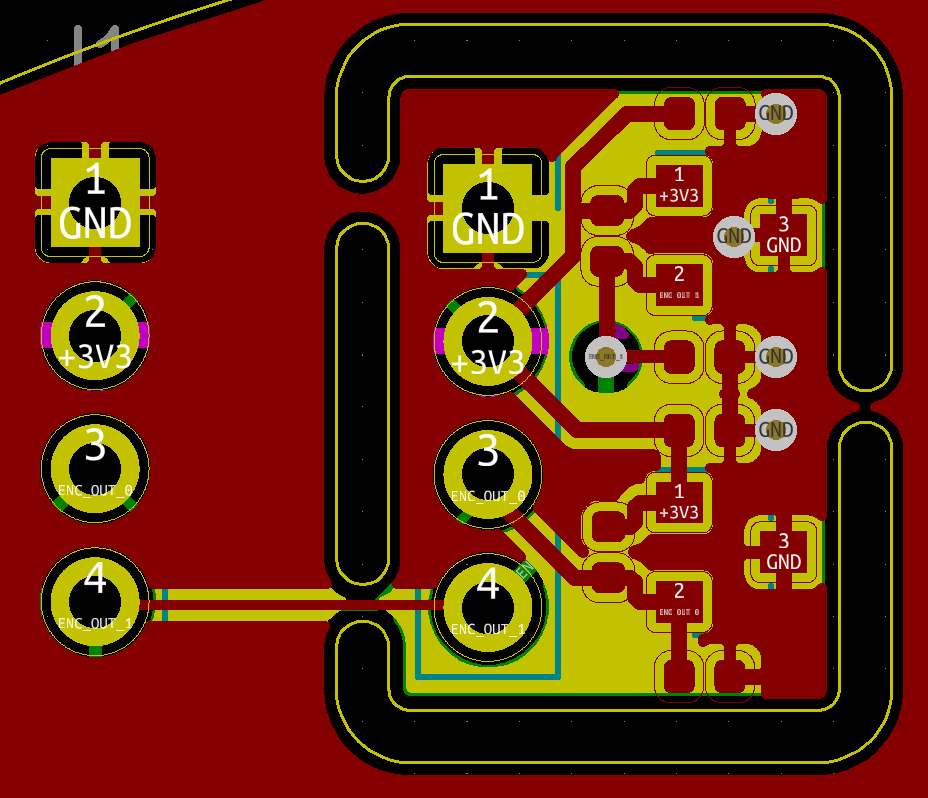
\includegraphics[width= 0.6\textwidth]{kapitoly/obrazky/E4/ir_motor_enkoder/pcb-enc.png}
    \caption{\label{fig:E4-enkoder_pcb}Vzhled enkorédu na desce}
\end{wrapfigure}
Aby bylo možno motor polohovat do správné polohy, je nutné mít zpětnou vazbu o~jeho poloze. Vzhledem k~tomu, že motor otáčí magnetem, samo se nabízí využít magnetický enkodér. 
Proto jsou na desce dvě digitální Hallovy sondy \href{https://datasheet.lcsc.com/szlcsc/Magnesensor-Tech-MST-MH253ESO_C114369.pdf}{MH253ESO}, které se překlopí podle toho, v jakém pólu 
se nachází. 

Na desce s~LED kruhem by sondy musely být na opačné straně než ledky, takže by se musely pájet ručně, protože JLCPCB osazuje jen z~jedné strany. Hlavní deska je ale zase, 
kvůli velikosti baterií, moc daleko od magnetu. 

Abych tedy nemusel dělat třetí desku jen kvůli enkodéru, zvolil jsem možnost vylomitelného enkodéru. Na hlavní desce jsem tedy nakreslil 
enkodér s konektorem a objel jsem ho frézou, aby se dal při montáži trezoru z desky vylomit a posunout do ideální polohy.

\begin{figure}[htbp]
    \centering
    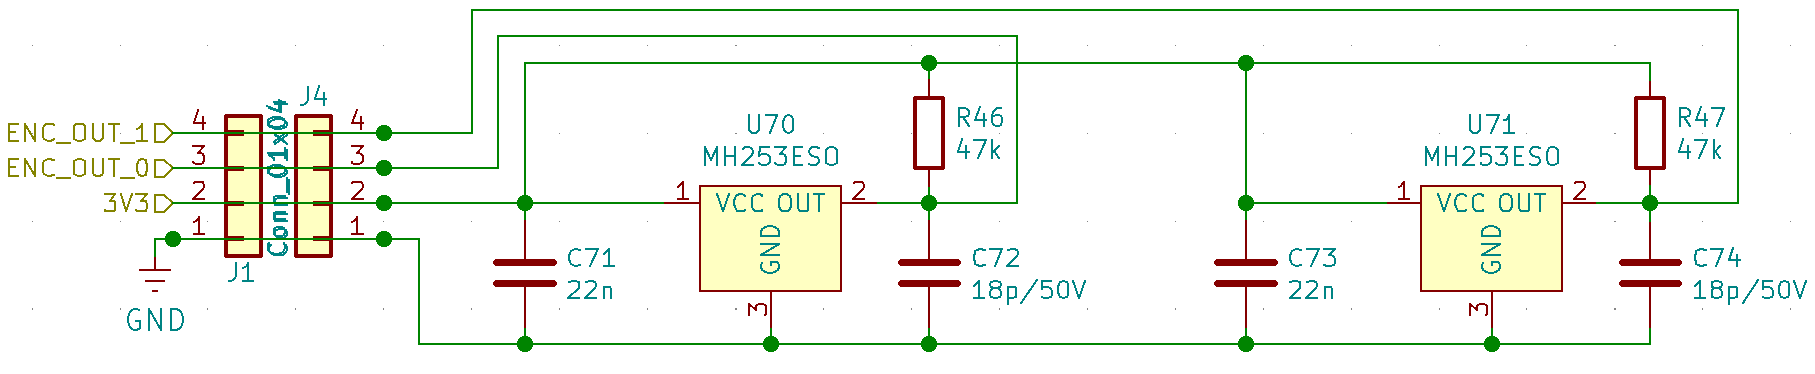
\includegraphics[width=\textwidth]{kapitoly/obrazky/E4/ir_motor_enkoder/enc.png}
    \caption{Zapojení enkodéru}
    \label{fig:E4-enkoder}
\end{figure}
